%%%%%%%%%%%%%%%%%%%%%%%%%%%%%%%%%%%%%%%%%%%%%%%%%%%%%%%%%%%%%%%%%%%%%%
% writeLaTeX Example: Academic Paper Template
%
% Source: http://www.writelatex.com
% 
% Feel free to distribute this example, but please keep the referral
% to writelatex.com
% 
%%%%%%%%%%%%%%%%%%%%%%%%%%%%%%%%%%%%%%%%%%%%%%%%%%%%%%%%%%%%%%%%%%%%%%
% How to use writeLaTeX: 
%
% You edit the source code here on the left, and the preview on the
% right shows you the result within a few seconds.
%
% Bookmark this page and share the URL with your co-authors. They can
% edit at the same time!
%
% You can upload figures, bibliographies, custom classes and
% styles using the files menu.
%
% If you're new to LaTeX, the wikibook is a great place to start:
% http://en.wikibooks.org/wiki/LaTeX
%
%%%%%%%%%%%%%%%%%%%%%%%%%%%%%%%%%%%%%%%%%%%%%%%%%%%%%%%%%%%%%%%%%%%%%%
\documentclass[twocolumn,showpacs,%
  nofootinbib,aps,superscriptaddress,%
  eqsecnum,prd,notitlepage,showkeys,10pt]{revtex4-1}

\usepackage{amssymb}
\usepackage{amsmath}
\usepackage{graphicx}
\usepackage{dcolumn}
\usepackage{xcolor}
\usepackage{marvosym}
\usepackage{url}
\usepackage{graphicx}
\usepackage{listings}
\usepackage{epigraph}


\definecolor{mygray}{rgb}{0.85,0.85,0.85}
 
\lstset{basicstyle=\ttfamily,
  showstringspaces=false,
  backgroundcolor=\color{mygray},
  basicstyle=\footnotesize,
  %commentstyle=\color{red},
  keywordstyle=\color{blue},
  captionpos=b,
  language=bash,
  basicstyle=\small\sffamily,
  numbers=left,
  numberstyle=\tiny,
  numbersep=3pt,
  frame=tb,
  columns=fullflexible,
  backgroundcolor=\color{gray!10},
  linewidth=0.9\linewidth,
  xleftmargin=0.1\linewidth
}
\usepackage[style=long,acronym,toc]{glossaries}
\usepackage{hyperref}
\hypersetup{
     colorlinks   = false,
     citecolor    = gray
}
\makeglossaries

\newacronym{hpc}{HPC}{'High Performance Computing'}
\newacronym{ib}{IB}{'InfiniBand'}
\newacronym{ui}{UI}{'User Interface'}
\newacronym{mpi}{MPI}{'Message Passing Interface'}
\newacronym{lxc}{LXC}{'LinuX Containers'}
\newacronym{nfs}{NFS}{'Network File System'}
\newacronym{hpcg}{HPCG}{'High Performance Conjugate Gradient'}
\newacronym{rhel}{RHEL}{'RedHat Enterprise Linux'}
\newacronym{cae}{CAE}{'Computer Aided Engineering'}
\newacronym{cfd}{CFD}{'Computational Fluid Dynamics'}
\newacronym{hpcac}{HPCAC}{'HPC Advisory Council'}
\newacronym{sysop}{SysOp}{'System Operations'}
\newacronym{openfoam}{OpenFOAM}{'Open Source Field Operation and Manipulation'}


%% Glossary
\newglossaryentry{slurm}{name=SLURM, description={Simple Linux Utility for Resource Management\footnote{\Mundus~\url{http://slurm.schedmd.com/}}}}
\newglossaryentry{elasticsearch}{name=Elasticsearch, description={Open-source text-index engine based on Lucene\footnote{\Mundus~\url{https://www.elastic.co/products/elasticsearch}}}}
\newglossaryentry{splunk}{name=Splunk, description={Commercial platform for Operational Intelligence\footnote{\Mundus~\url{http://www.splunk.com/}}}}
\newglossaryentry{graylog}{name=Graylog, description={Log management platform\footnote{\Mundus~\url{https://www.graylog.org/}}}}
\newglossaryentry{cgrp}{name=CGroups, description={Linux Control Grroups\footnote{\Mundus~\url{https://www.kernel.org/doc/Documentation/cgroups/cgroups.txt}}}}
\newglossaryentry{graphite}{name=Graphite, description={Metrics engine\footnote{\Mundus~\url{http://graphite.readthedocs.org/en/latest/}}}}
\newglossaryentry{logstash}{name=Logstash, description={powerful, modular event pipeline\footnote{\Mundus~\url{http://logstash.net/}}}}
\newglossaryentry{neo4j}{name=Neo4J, description={a graph database based on Lucene\footnote{\Mundus~\url{http://neo4j.com/}}}}
\newglossaryentry{osdc}{name=OSDC2014, description={Open Source Datacenter Conference 2014\footnote{\Mundus~\url{https://www.netways.de/?id=3132\#c27028}}}}
\newglossaryentry{ec}{name=EC, description={error code}}
\newglossaryentry{fqdn}{name=FQDN, description={Fully Qualified Domain Name}}
\newglossaryentry{nagios}{name=NAGIOS, description={Health check and alerting system widely used within the IT.}}
\newglossaryentry{openmp}{name=OpenMP, description={Open Multi-Processing, is an API that provides a shard memory among multiple servers.}}
\newglossaryentry{omp}{name=Open MPI, description={oMPI}}
\newglossaryentry{cos6}{name=CentOS 6.5, description={Community Enterprise Operating System in version 6.5, derived from the sources of Red Hat Enterprise Linux 6 (RHEL6).}}
\newglossaryentry{cos7}{name=CentOS 7.0, description={Community Enterprise Operating System in version 7.0, derived from the sources of Red Hat Enterprise Linux 7 (RHEL7).}}
\newglossaryentry{u12}{name=Ubuntu 12.04, description={Ubuntu 12.04.}}
\newglossaryentry{qdr}{name=QDR, description={Quad data rate (or quad pumping) is a communication signaling
        technique wherein data are transmitted at four points in the clock cycle:
        on the rising and falling edges, and at two intermediate points between them.}}

\newglossaryentry{rpm}{name=RPM, description={RPM Package Manager, a package management system created by RedHat. }}

\newglossaryentry{sriov}{name=SR-IOV, description={oMPI}}


\usepackage[printonlyused]{acronym}


\begin{document}

\title{An open and holistic framework to combine metric data, log events and inventory data.}
\author{Christian Kniep}
\affiliation{QNIB Solutions}

\begin{abstract}
IT infrastructure (no matter the size) is composed of multiple layers, supplied by different commercial vendors as well
as more and more open-source projects. This increasing complexity needs to be addressed by defining a common sense framework
to consume, process and explore the data produced by any part of the system; no matter if it is metrics data, event information or inventory data.

The pace of innovation is becoming faster and faster and thus the integration of new services has to keep up to speed. Long integration cycles
are going to be a handicap in a competitive, ever changing world.

In this paper a system is introduced, which serves as an open framework to consume, process, store and make use of
bits and pieces of information originating from each infrastructure layer.
The framework uses Docker as a foundation of a microservice architecture and integrates the best-of-breed open-source technologies
such as \gls{graphite}, \gls{logstash} and \gls{neo4j}.
This approach provides an inter-layer methodology which allows connections between subsystems like network,
software inventory and resource scheduler to assist in complex analysis of problems and performance. For example by correlating Infiniband
performance metrics with job-related information obtained from SLURM.
\end{abstract}

\maketitle


\section{Introduction}
% Placing the paper in the context of the discourse community and the field in general. Larger issue and debates are named
% and potentially problematised. In naming the location the writer is creating a warrant for their contribution and its 
% significances, as well as informing an international community of its relevance outside of its specific place of origin
%%%
% identified an issue and suggested that it is problematic and, by inference, that we have a different view.
% sometimes the locate work, e.g. will be more descriptive and sometimes more argumentative
% ..<topic>. is now a significant issue.. because...
%%%%%%%%%%%% what to put in
% Motivation
A data-center is comprised of a variety of different layers. From the physical hardware, support facilities (e.g. cooling) up to end-user applications.
Some of them are complex in themselves, yet every more ofter debugging a layer is impossible without taking information from connected part of the infrastructure into account.

One example is the interconnect, which provides communication between multiple entities.
A view into the layer itself provides information about data flows (bandwidth, latency) and errors on a switch and end-node basis.

As an system operator this angle might look appealing, but without a context in which the data flows occur the metrics are almost rendered useless, because
the correlation with information from other layers is put onto the shoulders of the operator.
He has to switch different tools with different User Interfaces and aspects to solve inter-layer problems.
% Model Switch and Transformation
\subsection{Model Discrepancy}
One aspect why the correlation of inter-layer information is such a hard task is a psychological one. Over time a human operator forms a mental model
of the system under his supervision. If information is received from somewhere, be it an event that occurred or performance metrics, this information
has to be mapped into the mental model which has been build so far.
The human is served best by a given tool, if the tools model and his mental model is completely aligned.
E.g. a hierarchical structure is displayed as a graph instead of a set of unconnected nodes.
This might be one reason why it is very common to recreate existing tooling around infrastructure projects (Not-Invented-Here syndrome), even though the underlying problem
is shared and equal among a broad spectrum of people. The driver seems to be that each system engineer has a slightly different model and prefers to build something from scratch.


% Interdisciplinary, open framework
This gets even worse in the complete infrastructure, since a variety of layers has to be covered, worst-case with different models even for common entities.
The network model only deals with host channel adapters and does not consider the actual host in his model (as InfiniBand does) in contrast to a resource
scheduler like \gls{slurm} (\glsdesc{slurm}) which only cares about hosts. Even this closely related topics, which are easily fit in a mental model, are hard to align in practice.
An even harder challenge is to model a commodity Ethernet network and align it with a special purpose interconnect like InfiniBand.
This leads to mostly distinct tools and even operational teams for different techniques within the IT infrastructure.

\subsection{Commoditization Problem}
While commoditization and specialization of hard- and software was one of the drivers to lower cost and the entry barrier to technology, it introduce an increase in layer count and
independent parts within each layer. The task to create an inter-layer framework became even harder and only tools like \gls{nagios} provided some insight.
The financial incentive to create an overarching framework which allows to mix, match and correlate information from different aspects is quite low, since the component vendors
do not benefit much from providing hooks to all tools out there.

\subsection{Open Framework}
To overcome this problem this work proposes an open framework embedded into a microservice architecture. The implementation aims for decoupled back-end, middle ware and front-end.
Inspired by the metrics ecosystem Graphite, which had this idea baked into the core from the beginning.


\section{Method}
\subsection{microservices}
The motivation behind this work dates back to the urge to run a complete HPC cluster stack in a visualized fashion on a single laptop in order to be able to gain a better understanding of how a HPC software stack interacts.
This first attempt was presented during the \gls{osdc} (\glsdesc{osdc}) 
All services were put into a single machine, which only served an environment needed to run the certain service.
Without calling it Micro-services the idea behind it was quite similar with the approach Micro-services are associated with.
One of the most quoted definition of the term Micro-services is served by Adrian Cockcroft:
\epigraph{Micro-services is defined as a loosely coupled service oriented architecture with bounded context}{\textit{Adrian Cockcroft}}
In practice the emerging pattern is that small team get full ownership of a particular service (bounded context).
How the service is implemented is of no interest to the clients (most likely micro-services themselves) of this service.
The interaction is strictly defined by a contract. A common protocol to provide this interaction is a RESTful API based on HTTP and JSON.

A litmus test of such an architecture is an update of services. 'Loosely coupled' should lead to a solution in which an update of one service
should not enforce an update to services using the API. If this test is passed successfully the system provides
independent update cycles for each service, without breaking the current system as a whole.


\subsection{Service Discovery}
When implementing a microservice architecture the amount and scale of services can become a big burden when it comes to coupling the services.
If hooking services together implies manual labor to put IP addresses into configuration files, the scalability of the system is going to be fairly limited.
Instead, the system should advertise its capabilities and discover other services automatically.

The used implementation started as a set of bash scripts updating \gls{etcd} (\glsdesc{etcd}).
This key/value store was used by \gls{skydns}, which exposes entries
over a DNS interface and thus made the coupling of distributed services relatively easy. To dynamically create configuration files a tool called
\gls{confd} (\glsdesc{confd}) emerged, which queries \gls{etcd} and produces configuration files from templates if a watched value changes.

A more holistic tool to deal with this set of functionality is \gls{consul} (\glsdesc{consul}). It combines a key/value store, service checks,
a DNS interface and an RESTful API in one golang binary, which is easy to manage.

\autoref{lst:srv_json} shows an example of a service, including attributes and checks to determine the state of the service based on the return code of the script (like NAGIOS does). 

\begin{lstlisting}[language=bash,
    caption={Service definition within \gls{consul}. If the keyword \texttt{open} is not found within the nmap output the service is set into a warning state.},
    label={lst:srv_json}]
{
  "service": {
    "name": "nginx",
    "port": 80,
    "check": {
      "script": "nmap 127.0.0.1 -p80|grep open",
      "interval": "10s"
    }
  }
}
\end{lstlisting}

If the check indicates the service is usable, the service is exposed via an DNS interface.
Thus the service can be reached via the \gls{fqdn} (\glsdesc{fqdn}) \lstinline{<service-name>.service.consul}
as shown in the example in \autoref{lst:dig_nginx}.
\begin{lstlisting}[language=bash,
    caption={DNS query of \lstinline{nginx} service, issued with \texttt{dig}, a common DNS resolver.},
    label={lst:dig_nginx}]
$ dig SRV +short nginx.service.consul
1 1 80 nginx.node.consul.
\end{lstlisting}

The ablility to reference a service via DNS is extremely helpful, since name resolving works system-wide. Instead of static IP address,
a configuration file contains the \gls{fqdn} to describe a dependency to a different node. Furthermore the complete tooling
is going to work as well; checking network connectivity is as simple as using \lstinline{ping} to resolve the \gls{fqdn}.

\autoref{lst:curl_nginx} shows an example of the RESTful API to access information as JSON blobs.

\begin{lstlisting}[language=bash,
    caption={Exposure of services via RESTful API.},
    label={lst:curl_nginx}]
$ export URL=localhost:8500/v1/catalog/service
$ curl -s $URL/nginx|python -m json.tool
[
    {
        "Address": "172.17.0.6",
        "Node": "nginx",
        "ServiceAddress": "",
        "ServiceID": "nginx",
        "ServiceName": "nginx",
        "ServicePort": 80,
        "ServiceTags": null
    }
]
\end{lstlisting}
This provides the ability to use this information in external scripts or use the rich ecosystem that has already build up around service discovery.

Since this work aims to be modular and flexible in its composition, a service discovery mechanism which is able to dynamically update itself is crucial to the success of the framework.


\subsection{Linux Container}
The current wave of OS-level virtualization leverage Kernel Namespaces to isolate different groups of processes. Unlike hypervisor visualization, which emulates
the hardware of a physical computer, OS-level virtualization are spawning processes with certain flags, attaching the process (and its children's processes)
to a set of namespaces. The Linux Kernel provides Kernel Namespaces to encapsulate processes, mount points, network stacks,
inter-process communication and domain information. Furthermore a container can be granted only a subset of kernel capabilities.

A common way to restrict the use of resources (CPU, memory, I/O) available by a running container is the use of \gls{cgrp} (\glsdesc{cgrp}).

\subsubsection{Linux Containers}
An early contender to OS-level virtualization FreeBSD `jails', Solaris `Zones' and \gls{lc}. They never gained much momentum, since they had operational limitations are were a bit cumbersome to use.

\glspl{lc} are a perfect fit for a microservice architecture. They do not spin up a complete operating system but only the process
necessary for the service and therefore minimize the overhead. Furthermore \glspl{lc} are started and stopped within a
fraction of a second, which provides a proactive elasticity needed to be agile.

\subsubsection{Docker}
The \gls{lc} implementation that took off within the last couple of months is Docker. It leads the rise of \glspl{lc} as a commodity technology, accessible
for a broad range of users. It provides an easy and intuitive way to build, distribute and run container images.
By developing Docker in the open and providing an API, Docker gained a lot of momentum and surrounded Docker with a rich ecosystem.

\subsubsection{Containers versus Virtual Machines}
One could argue that virtual machines are best suited to serve monolithic applications,
which assume an uninterrupted operation. If the underlying hardware is failing the virtual machine gets migrated to a different host. Ideally just
with a slight hiccup, while the network address is transferred. The application itself is designed to life a long and protected life.

In the microservice architecture dealing with failure is a crucial part of the design itself. A system should not have single points of failure and
should self-heal if a service fails. How many (and which) concurrent errors a system can withstand depends on the effort put into it and might differ
in certain stages of the development, but the ideal goal is a self-healing system.




\subsection{Metrics Engine and Log Pipeline}
Unlike metrics, which are data-points associated in a time series (most are repetitive, like system performance information)
fashion, log data is a distinct event. Granted, the line is a bit blurry and some events include metric data that
might be extracted in a subsequent step. NAGIOS e.g. provides performance information with most of the alarm events to enrich the event.

In an ideal world the two would be separated pieces of information. A metric does not provide context
but pure distilled performance information in the form of a value connected to a metric key and timestamped.

A log event would be pure context without any performance information (e.g. 'Cronjob to sync video data started by user bob'). 

In practice the producer of an event is most likely to cross this line, since the past favored an enriched (human readable/understandable) event over a
pure piece fed into the correlation engines of today. But today this line gets redrawn; in times were big data is a hype topic for the last couple
of years, the quality/clarity/focus of incoming data matters.

\subsubsection{Metrics Engine}
The first pillar of the open framework is the metric engine ecosystem Graphite, which captures performance values over time. 
First released in 20xx it provides a modular system to consume, process, store and access metric information in the form 'key value time-stamp'.

The metrics are persisted in round-robin databases called whisper by a set of daemons called 'carbon'.

\begin{lstlisting}[language=bash,
    caption={Sending and receiving metrics using carbon in combination with a whisper file back-end.},
    label={lst:carbon_wsp}]
$ for x in {1..5};do
> echo "test.metric ${x} $(date +%s)" |\
    nc -w 1 127.0.0.1 2003
> sleep 5
> done
$ export CDIR=/var/lib/carbon/whisper
$ whisper-fetch $CDIR/test/metric.wsp |\
    grep -v None
1438513460	1.000000
1438513465	2.000000
1438513470	3.000000
1438513475	4.000000
1438513480	5.000000
$
\end{lstlisting}

The graphite framework provides a rich ecosystem of visualizations, plugins, metric sources and alternative daemon implementation to fit almost
all use-cases around metrics gathering, processing, storing and serving metrics. Due to its open-source development and defined API missing pieces
can be added if needed.

This enables each part of the infrastructure layer to submit it's metrics. Even application developers can just start sending metrics down the pipeline and
let them pop up at the access layer.

- Metric Key Scheme

If the group of metric generators grows to a certain complexity the metrics keys becoming a problem, since naming schemes vary depending on the context of
the producer. An engineer overseeing the network in a data-center might organize his metrics hierarchical (\lstinline{datacenter01.rack01.compute01.eth0.send_bytes}), while from the
resource scheduler perspective a grouping per job ($jobid01.compute01.send\_bytes$) is a scheme which might fit the use-case best.

To overcome this issue a scheme should be chosen which describes the metric in a deterministic and unique way. This ID is then logically structured according to the use-case.
Concepts like Metrics 2.0\footnote{\Mundus~\url{http://metrics20.org/}} (shown in \autoref{lst:metrics20}) annotate metrics with metadata.

\begin{lstlisting}[language=bash,
    caption={Metrics2.0 formatted metric},
    label={lst:metrics20}]
{
    server: dfs1
    what: diskspace
    mountpoint: srv/node/dfs10
    unit: B
    type: used
    metric_type: gauge
    value: 1024
}
meta: {
    agent: diamond,
    processed_by: statsd2
}
\end{lstlisting}

\subsubsection{Log Pipeline}
In the past Log engines like \gls{splunk} (\glsdesc{splunk}) were high priced data consumers, which proposed to help deal with the
flow of incoming unstructured data. Without such a framework it was very hard to normalize all the data and make use of the information gathered.

In the last couple of years open-source tools emerged. The most prominent is \gls{logstash} (\glsdesc{logstash}),
followed by \gls{graylog} (\glsdesc{graylog}).
They provide a modular pipeline, which allows to take data from different inputs, normalize it (commonly in some JSON-style format)
and alter the information on the way through. Among others the data is then persisted in a data-store, e.g. in \gls{elasticsearch} (\glsdesc{elasticsearch}).
Both ecosystems provide visualization tools and connectors to a rich ecosystem.

\begin{lstlisting}[language=bash,label={lst:ls_cfg},
    caption={Basic Logstash configuration}]

input {
    syslog {
        port => 5514
        type => syslog
    }
}
filter {
    mutate {
        add_tag => [ "special" ]
    }
}

output {
    stdout { codec => rubydebug }
}
\end{lstlisting}

The power of these pipelines lies in the flexibility they provide. With a couple of lines (an example is shown in \autoref{lst:ls_cfg}) of
configuration the logs are centralized and accessible via an intuitive dashboard like \gls{kibana}\glsdesc{kibana} as they were never before. Compared to plain text files on each server itself this changes the way logs are correlated with each other.



\subsection{Inventory}
Existing inventory systems face a twofold problem. First they are mostly designed for one particular layer of the infrastructure cake.
This burdens certain constraints to the model of the system, which are hard to overcome. A holistic approach is very rare, some might
provide a global character, but most likely as an historically grown extension.

The second problem comes down to the technique used. Most systems use some sort of Rational Database, which has a tendency to normalize
the schema involved to eliminate redundant information. Once a schema is set up, it is hard to shoehorn other aspects of the data-center into
the established schema formed by the first consideration.

To overcome this, the system should be backed by a graph database, which allows a schema-free model to evolve over time. Different aspects
use different models. Inter-layer dependencies are modeled by connecting the related nodes. This allows a rich query to span across multiple layers.


\subsection{OpenSM}
The management of InfiniBand is centralized and coped with by one daemon per subnet. This service holds the inventory,
computes the routing tables for each switch, reacts on events within the network, etc.
The OpenFabrics Alliance\footnote{\Mundus~\url{http://www.openfabrics.org/}} provides an open-source implementations called OpenSM\footnote{\Mundus~\url{http://git.openfabrics.org/}}.


Fabriscale\footnote{\Mundus~\url{http://fabriscale.com/}} has extended OpenSM,
to provide better routing capabilities alongside with enhancements in operational aspects.
By providing a RESTful API, the daemon \texttt{fabriscale} is a good fit to be integrated in
a microservice architecture. Furthermore it provides a plugin to extract performance information and send these off to the metrics engine.


\subsection{QNIBMon}
To provide a holistic, multi-layered approach to infrastructure management the proposed framework combines
all of the presented techniques.
An open metric engine, log event pipeline and inventory system based on a graph database.
All of this held together using \texttt{Consul} as a service discovery
tool.
The microservice architecture comprises of the services shown in \autoref{fig:qnibmon_arch}.
\begin{figure}[!ht]
    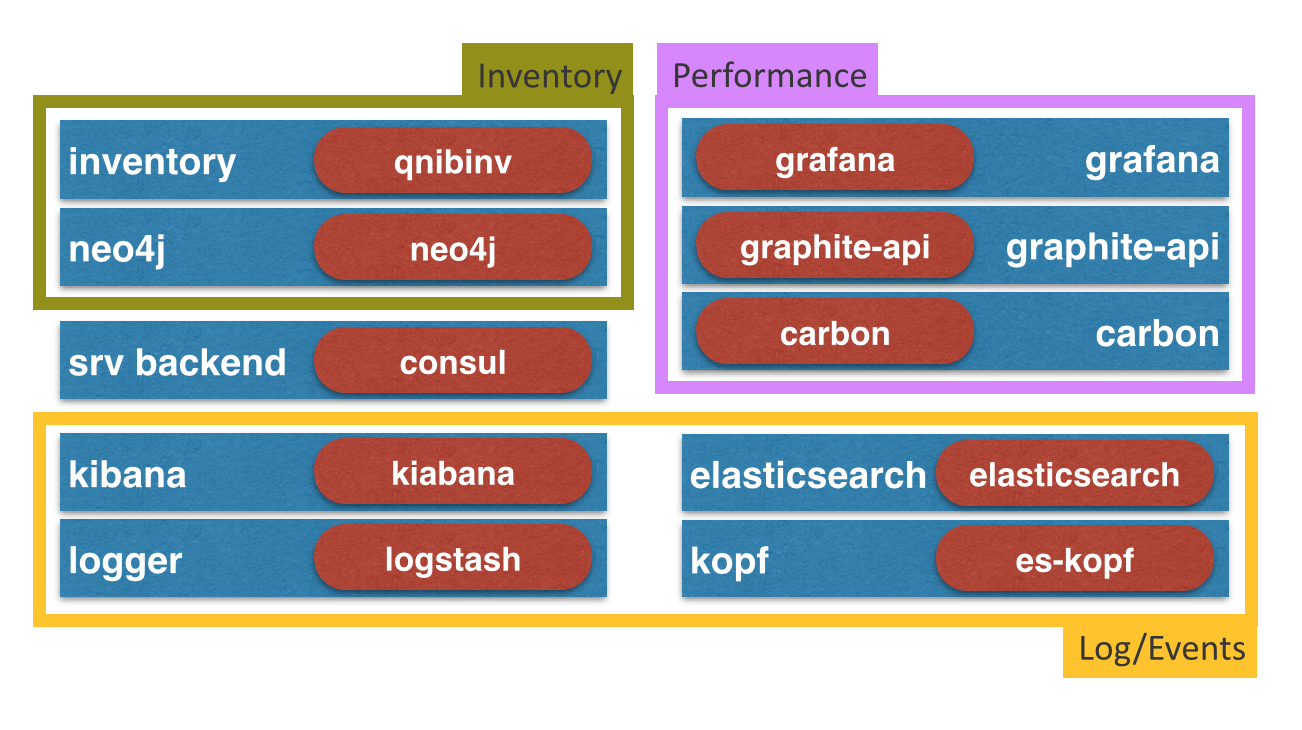
\includegraphics[width=.4\textwidth]{images/png/qnibmon_arch.png}
    \caption{\label{fig:qnibmon_arch}Composition from a container and service view}
\end{figure}



\section{Correlating InfiniBand and SLURM}
By combining the presented technology stacks, the framework provides deep insights into the complete cluster stack.

\subsection{Domain Modeling}
By using a schema-less graph database approach, each domain can be modeled independently. Common entities are connected at any time after
they are modeled.

\subsubsection{Resource Scheduler}
\gls{slurm} provides information about resource allocations: Which jobs was started where, by whom at what time? How long did it last? What was the outcome? and alike.
The following \gls{slurm} entities are modeled as nodes within the graph.
\begin{itemize}
    \item \textbf{host} The \gls{slurm} node, which represents a compute node within the cluster, identified by the host-name.
    \item \textbf{partition} A logical group of nodes which represent the target of a job submission.
    \item \textbf{job} A demand for resources submitted by a user. Including metadata (user, submission/start/end time, job script, etc) and information about the state of the job. If resources are allocated, the job metadata is updated accordingly.
\end{itemize}
Relationships are added to connect certain nodes. \lstinline{PART_OF} declares host memberships to partitions. \lstinline{JOBCLIENT} connects a host to a certain running job.

\subsubsection{InfiniBand Interconnect}
An InfiniBand representation comprises of a set of physical and logical representations.
\begin{figure}[!ht]
    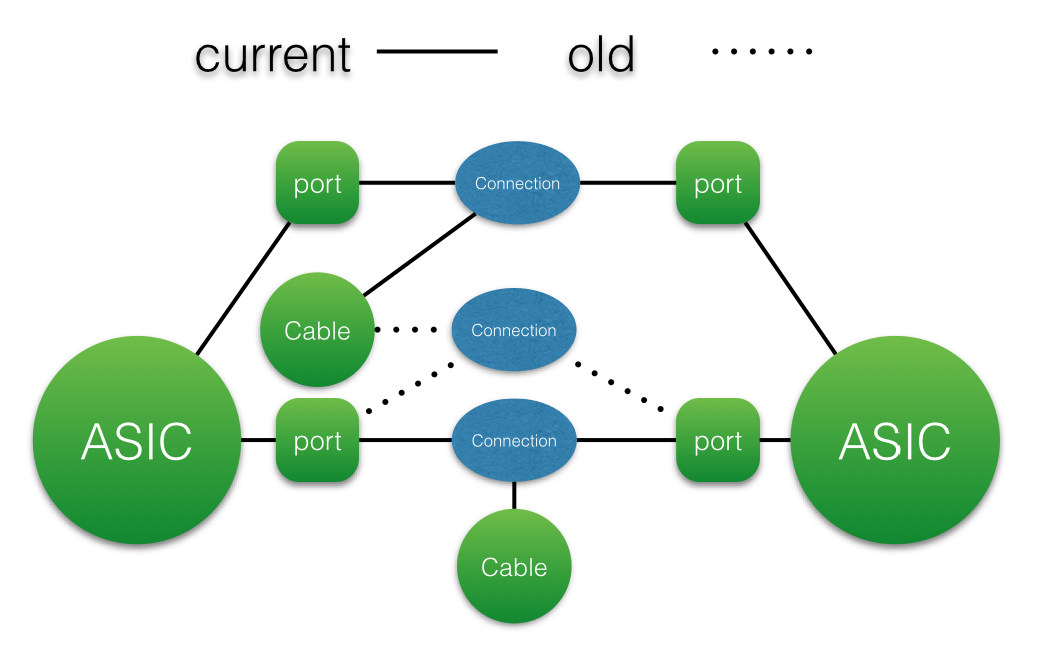
\includegraphics[width=.4\textwidth]{images/png/infiniband_graph.png}
    \caption{\label{fig:ib_graph}Modeling of an InfiniBand network.}
\end{figure}

\begin{itemize}
    \item \textbf{HCA} Network adapter plugged into a host
    \item \textbf{SW} InfiniBand switch
    \item \textbf{PORT} Each \lstinline{HCA} and \lstinline{SW} are composed of a set of ports which provide connectivity.
    \item \textbf{CABLE} Physical connection between different ports.
    \item \textbf{CONNECTION} Logical entity which connects two \lstinline{PORTS} and a \lstinline{CABLE} for a given period in time.
\end{itemize}

Relationships combine two \lstinline{PORTS} and a \lstinline{CABLE} alongside with meta-information about the time when it was created, if the connection is still valid and a like.
Furthermore the routing information is added by providing a \lstinline{ROUTE_TO} relationship between a port and a host.

\subsection{Holistic Inventory}
The presented two models alone provide combined insight into the cluster. By connecting the HCA (within the InfiniBand model) to a host (within the \gls{slurm} model) the inventory allows inter-layer queries.

\subsubsection{Job Placements}
By showing the layout of a job within the \gls{ib} topology, an imbalanced job is easily detectable. \autoref{fig:hop_mis} shows an example in which the hop-count within a job differs.
\begin{figure}[!ht]
    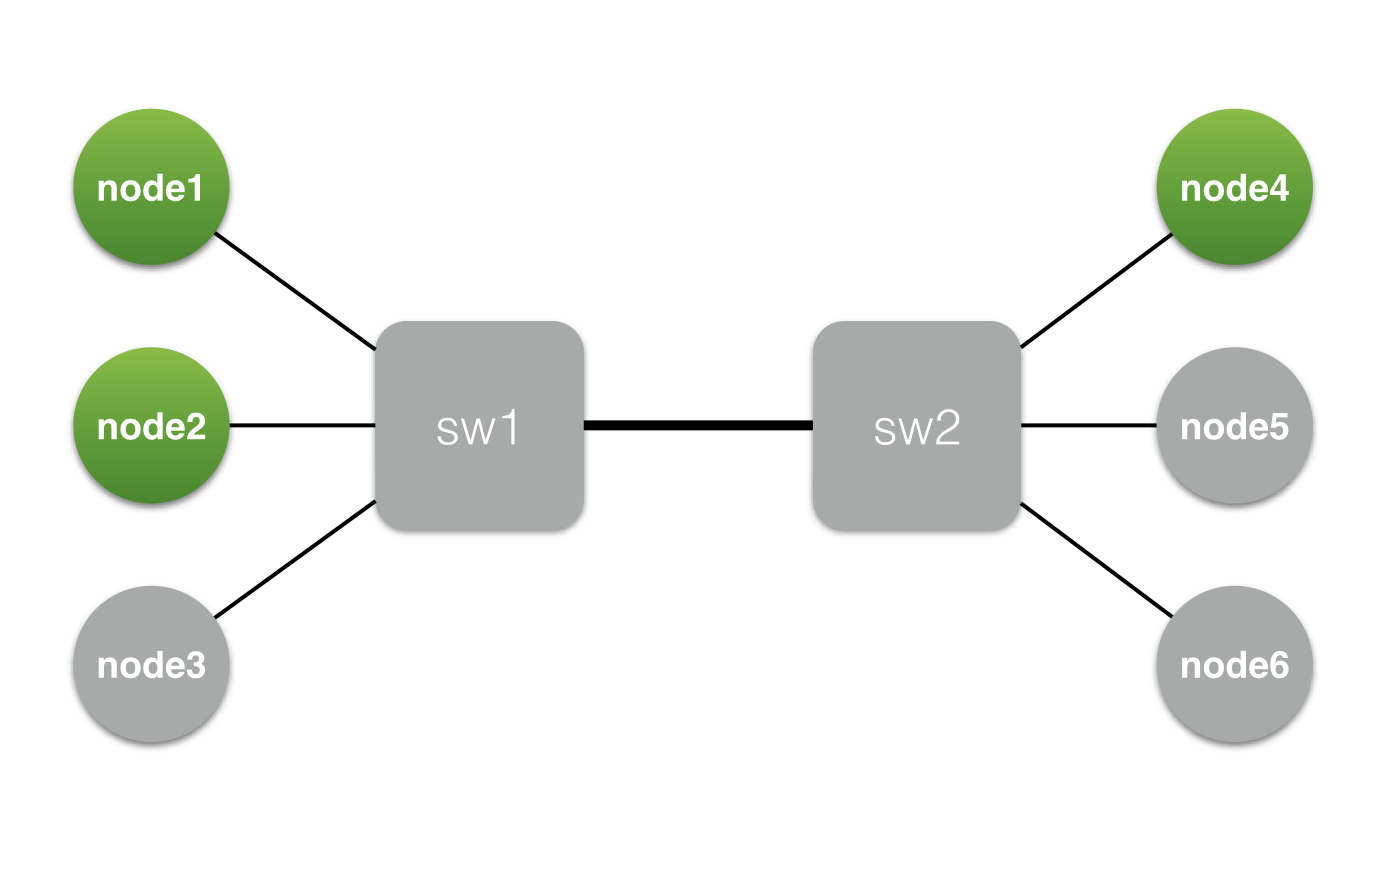
\includegraphics[width=.4\textwidth]{images/png/hop_missmatch.png}
    \caption{\label{fig:hop_mis}A job runs on three nodes (green). By using \lstinline{node3} instead of \lstinline{node4} the job could run evenly distributed on \lstinline{sw1}}
\end{figure}
A slightly more complex case would include different port-characteristics like speed, width.
By caching information of the metrics system within the ports an even more sophisticated query might include error or performance counters.

\subsubsection{InfiniBand Debugging}
A common debug case within the InfiniBand network is to figure out if errors associated with a connection are caused by one of the ports or the cable itself.
The approach to fix this error is to carefully unplug one connector of a given cable, connect it to a different switch-port and check the error counters of the just established connection.
If the error sticks with the cable the opposite side of the cable has to be changed as well, to truly pin down the problem.

This process is extremely error prone; an inventory to deal with an InfiniBand fabric barely exists. Therefore each step is manual labor with the risk of miscommunication between the on-site engineer changing the
cables and the engineer matching the changes to performance counter changes.

By using an holistic inventory (as indicated in \autoref{fig:ib_graph}) the changes are tracked automatically and since they include the timestamps the correlation with the metrics systems is trivial.

\subsection{Open Log and Metric Framework}
Determining inter-layer error triggers is an extremely hard task. If e.g. a specific job triggers an error within the interconnects one has to keep track of the job placement, the routes within the interconnect and
the time to correlate metrics with this events.

\begin{figure}[!ht]
    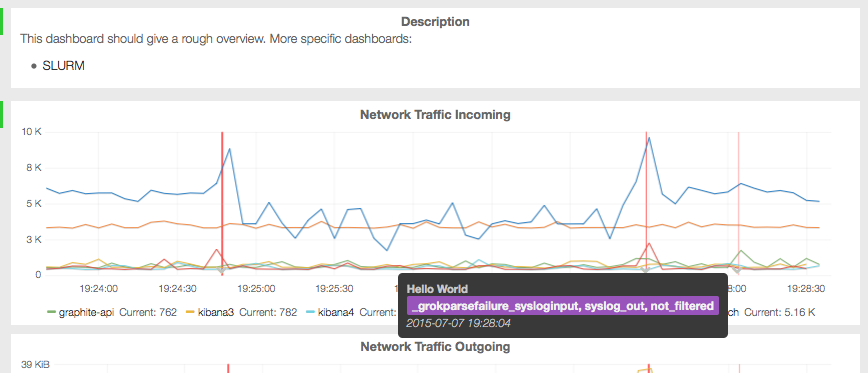
\includegraphics[width=.4\textwidth]{images/png/mon_cor.png}
    \caption{\label{fig:job_correlation}Correlation of performance metrics and job events.}
\end{figure}
\autoref{fig:job_correlation} shows the performance metrics annotated with job events, which provides an easy to spot correlation between the two domains.



\section{Future Work}

The coupling of metrics, log events and inventory data is still an area which is researched and therefore it is not battletested.

\subsection{Data Back-end}
When talking to different camps within the space it seems that each back-end is a good fit to cover all needs.
Some say, it is safe to store metric information in Elasticsearch. On the other hand InfluxDB supports storing events and so on.

In the future the right balance, back-end and connectivity has to be found.

\subsection{Metrics 2.0}
Aligning the metrics2.0 concept to allow tighter and more specific reference of tags might help connect information.
Tags might implicitly describe to which data-point (inventory or event) they are referring to.

\subsection{Inventory Model}
More domain models have to be included into the Inventory system to gain more experience in regards of possible friction points and limitation to this approach.

\subsection{Scale Test}
The use of this framework is so far limited to small clusters and a laptop. How well it is going to scale and what the limitations are is to be discovered.


\section{Conclusion}
Overall, this approach provides a framework which allows rapid prototyping and integration of services.
By leveraging the service discovery the configuration overhead is minimized and the software stack configures itself for the most part.

Due to its modularity the framework is an optimal contender to integrate new services without interfering with existing parts.
The microservice architecture implicitly forces well defined interactions in between the subparts, which allows to remove, add or duplicate functionality if needed.
Incoming metrics for example might be mirrored and send to a backend system for evaluation without breaking existing queries.

By using a schema-less graph database as inventory system, domains can be modeled separatley and connected as a subsequent step. This allows inter-layer
correlation without the need to define a least common denominatior beforehand.

Kibana as the main log event dashboard and Grafana as the initial performance metric visualization provide
state-of-the-art flexible and intuitive access to the information stored in the complete infrastruture stack.
By leveraging the inventory information dashboards are generated automatically to provide up to date views.


While not tested at scale the system works nicely as a testing environment. All subsystems are known to scale horizontally.


%\section{Glossary}
%\printglossaries

\begin{acknowledgments}
\end{acknowledgments}



\end{document}